%!TEX TS-program = xelatex
%!TEX engine = xelatex

\documentclass{standalone}

\usepackage{fontspec}
\setmainfont{Fira Mono}
\usepackage{unicode-math}
\setmathfont[Scale=MatchUppercase]{STIX Two Math}
\setmathrm[Scale=MatchUppercase,
           BoldFont=STIX Two Text Bold]{STIX Two Math}
\setmathtt[Scale=MatchUppercase]{Fira Mono}

\usepackage{tikz}

\begin{document}
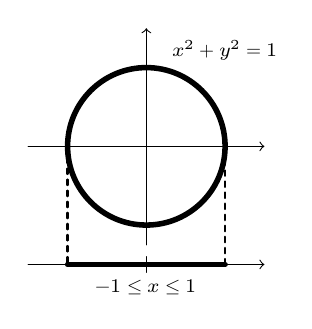
\begin{tikzpicture}[line cap=round,line join=round]
  \draw[->,color=black] (-1.5,0.) -- (1.5,0.);
  \draw[->,color=black] (-1.5,1.5) -- (1.5,1.5);
  \draw[->,color=black] (0.,0.25) -- (0.,3);
  \draw (0, -.1) -- (0, .1);
  %\clip(-1.5,-0.5) rectangle (1.5,3);
  \draw [line width=2.pt] (0.,1.5) circle (1.cm);
  \draw [line width=0.8pt,dash pattern=on 2pt off 2pt] (-1,1.5)-- (-1.,0.);
  \draw [line width=0.8pt,dash pattern=on 2pt off 2pt]
        (1.,0.) -- (1,1.5);
  \coordinate (c) at (1, 2.5);
  \draw [line width=2.pt] (-1.,0.)-- (1.,0.);
  \begin{scriptsize}
    \draw[color=black] (c) node[above, anchor=south] {$x^2 + y^2 = 1$};
    \draw[color=black] (0, -.1) node[below, anchor=north] {$-1 ≤ x ≤ 1$};
  \end{scriptsize}
\end{tikzpicture}
\end{document}
